\chapter{Using Disks and Disk Images}
\label{cha:using-disks}

\phantomsection

\section{Disk Drives}
\index{Disk Drives}

The MEGA65 has a built-in 3.5" floppy disk drive, and supports Commodore-style external disk drives via the IEC serial port on the back of the computer. The IEC port also supports other external IEC storage devices, such as the SD2IEC. Some IEC storage devices can be connected in a chain and used at the same time.

The MEGA65 also includes a ``virtual'' disk drive that can mount D81 disk image files stored on the SD card. Most MEGA65 software that you download from the Internet is in the form of a D81 disk image. You can create a new D81 disk image directly from the MEGA65, and start saving your BASIC programs to the SD card without any additional hardware. You can also copy files between physical floppy disks and D81 disk images.

The Intro Menu that you saw when you first switched on the computer is a program on a D81 disk image, a file named {\tt MEGA65.D81} on the SD card. The MEGA65 is initially configured to boot this disk image automatically. You can change this in the Configuration Utility. (Refer back to chatper \vref{cha:configuringyourmega}.)

You can manage disk drives and virtual disk images from the Freezer menu. Some of these operations can be performed with BASIC commands such as {\bf MOUNT}.

\subsection{Unit Numbers and Drive Numbers}
\index{Disk Drives!Terminology}
\index{Connections!IEC}

Each disk drive (physical or virtual) is accessed via a {\it unit} number. With vintage Commodore computers, the unit number refers to an IEC device connected to the computer. Commodore reserved unit numbers in the range 0 -- 31 for devices of various purposes, with 8 -- 11 reserved for disk drives. If you've ever used a Commodore 64 and typed \screentext{LOAD "*",8,1}, the ``8'' refers to the disk drive connects as unit 8. BASIC 65 disk commands use unit 8 by default, and accept a {\bf U} parameter to change it, such as: \screentext{DLOAD "MYPROGRAM",U9}

With the MEGA65, you can assign a unit number to the virtual disk drive with a D81 disk image mounted, or to the internal 3.5" floppy drive. You must ``mount'' a disk image or the internal 3.5" floppy drive to a unit number before it can be used. Any message sent to a unit number assigned to a virtual disk or the internal floppy drive is handled by the MEGA65. All other messages are sent to the IEC serial port.

Disk commands also accept an optional parameter to specify a {\it drive} number. This is only needed when connecting a vintage dual floppy drive via the IEC port, such as the Commodore 4040, 8050, or 8250. Every disk drive assigns drive number 0 to the first drive. Dual-drive units assign a drive number of 1 to the second drive. Dual disk drives are usually equipped with an IEEE-488 interface, and need an IEEE-488 to IEC converter to be used on the MEGA65. BASIC 65 disk commands use device 0 by default, and accept a {\bf D} parameter to change it.


\section{Using Virtual Disk Images}

The MEGA65 provides a virtual disk drive that uses D81 disk image files from the SD card. The virtual drive behaves like a Commodore 1581 drive, without the need for vintage physical media.

You can mount up to two virtual disks at a time, or one virtual disk and the internal 3.5" floppy drive. Each virtual disk can be assigned to unit 8 or 10, and 9 or 11.

\subsection{Where to Get Disk Image Files}

The MEGA65 Filehost website hosts a library of MEGA65 software produced by the community. You can browse or search for software, download a title, then copy the D81 disk image to the SD card using either your PC or the Ethernet file transfer tool.

\url{https://files.mega65.org/}

\subsection{Mounting Disk Images with the Freezer}

Open the Freezer menu: hold \widekey{RESTORE} for one second, then release it. Notice the current drive mounting settings in the lower-right of the screen.

\begin{center}
  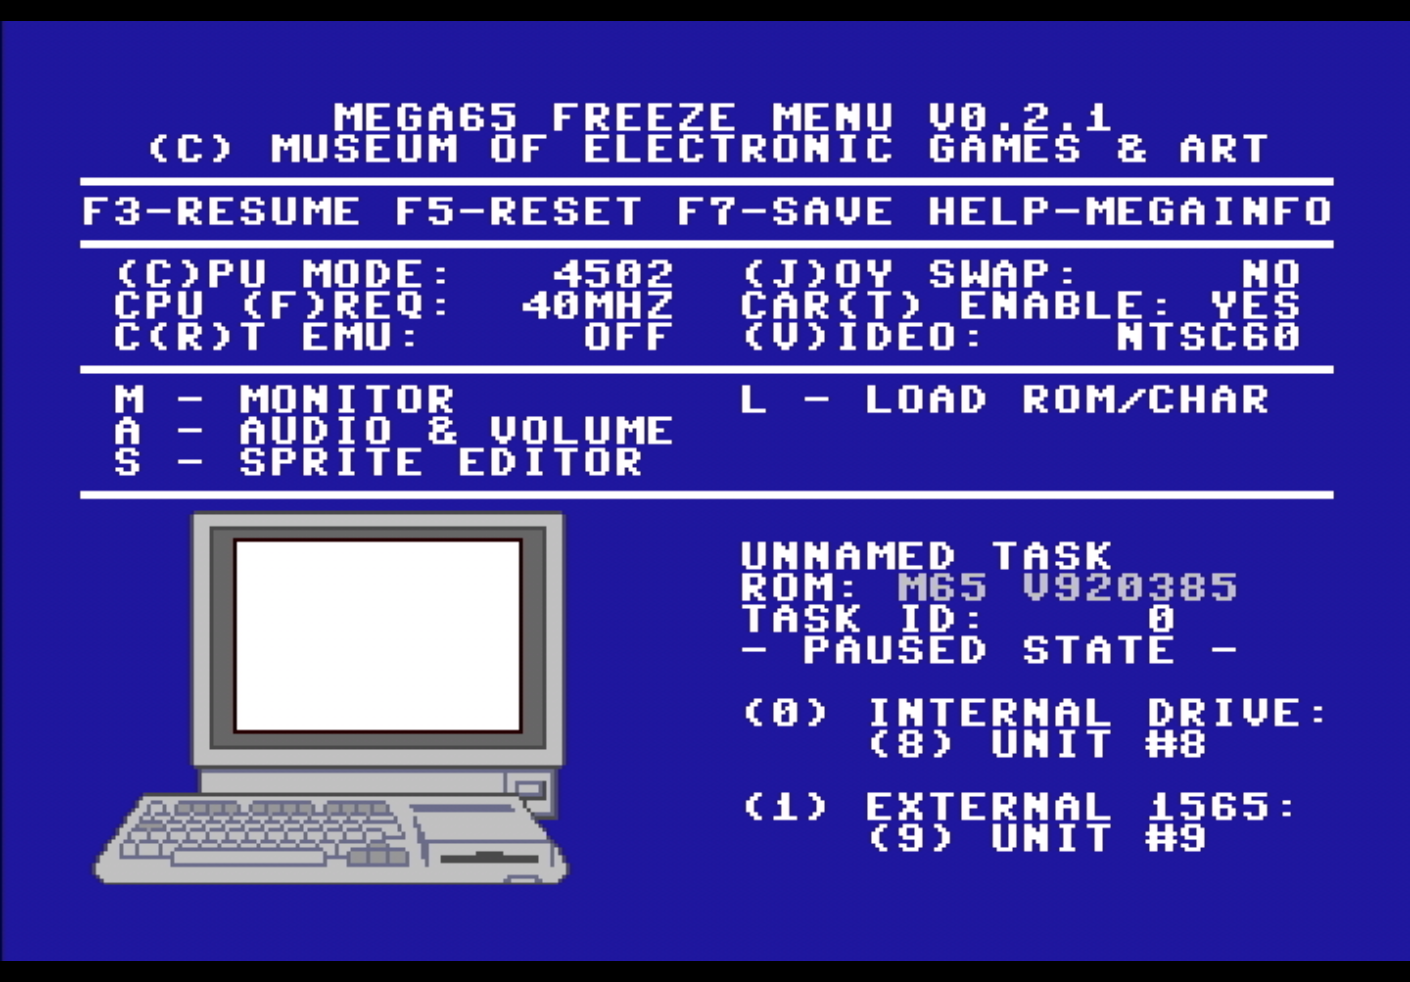
\includegraphics[width=0.7\linewidth]{images/freezer.png}
\end{center}

To mount a disk image on unit 8 or 10, select the first managed drive by pressing \megakey{0}. To mount a disk image on unit 9 or 11, select the second managed drive by pressing \megakey{1}. This opens the SD card file browser.

\begin{center}
  \includegraphics[width=0.7\linewidth]{images/d81-file-browser.png}
\end{center}

Using the cursor keys to select a D81 disk image, then press \widekey{RETURN}. The Freezer screen shows the selected disk image is now associated with the managed drive.

From the main Freezer screen, press \megakey{8} or \megakey{9} to toggle the unit number assigned to the first or second managed drive, respectively.

\subsection{Mounting Disk Images from BASIC}

The BASIC {\bf MOUNT} command can mount a D81 disk image from the SD card without having to open the Freezer. This command can be entered at the \screentext{READY} prompt, or be used as part of a program.

To mount a disk image on unit 8, enter {\bf MOUNT} with the full filename in double-quotes, including the {\tt .D81} suffix:

\begin{screenoutput}
MOUNT "MEGA65.D81"
\end{screenoutput}

To mount a disk image to unit 9, 10, or 11, also provide the {\bf U} argument:

\begin{screenoutput}
MOUNT "MEGA65.D81",9
\end{screenoutput}

\subsection{Creating a New Disk Image}

You can create a new empty disk image from within the MEGA65 Freezer.

\begin{enumerate}
\item Open the Freezer.
\item Press \megakey{0} to select the first managed drive.
\item At the top of the file list, select: \screentext{- NEW D81 DD IMAGE -}
\item When prompted, enter a name for the disk. (Omit the {\tt .D81} suffix; this will be added automatically.)
\end{enumerate}

The new disk image is created on the SD card and mounted to the first managed drive. It is formatted and ready to use.

\subsection{Managing SD Card Files in Sub-directories}

Once you have spent some time on Filehost downloading games and apps, you will eventually have a large collection of D81 disk images on your SD card. You may wish to organize these files into sub-directories (folders). You can create these folders with the SD card connected to your PC, or with the Ethernet file transfer tool.

The Freezer supports sub-directories in its file browser. Each sub-directory name begins with a slash ({\tt /}). Select a folder to visit it. To return to the previous folder, select {\tt /..}.

\begin{center}
  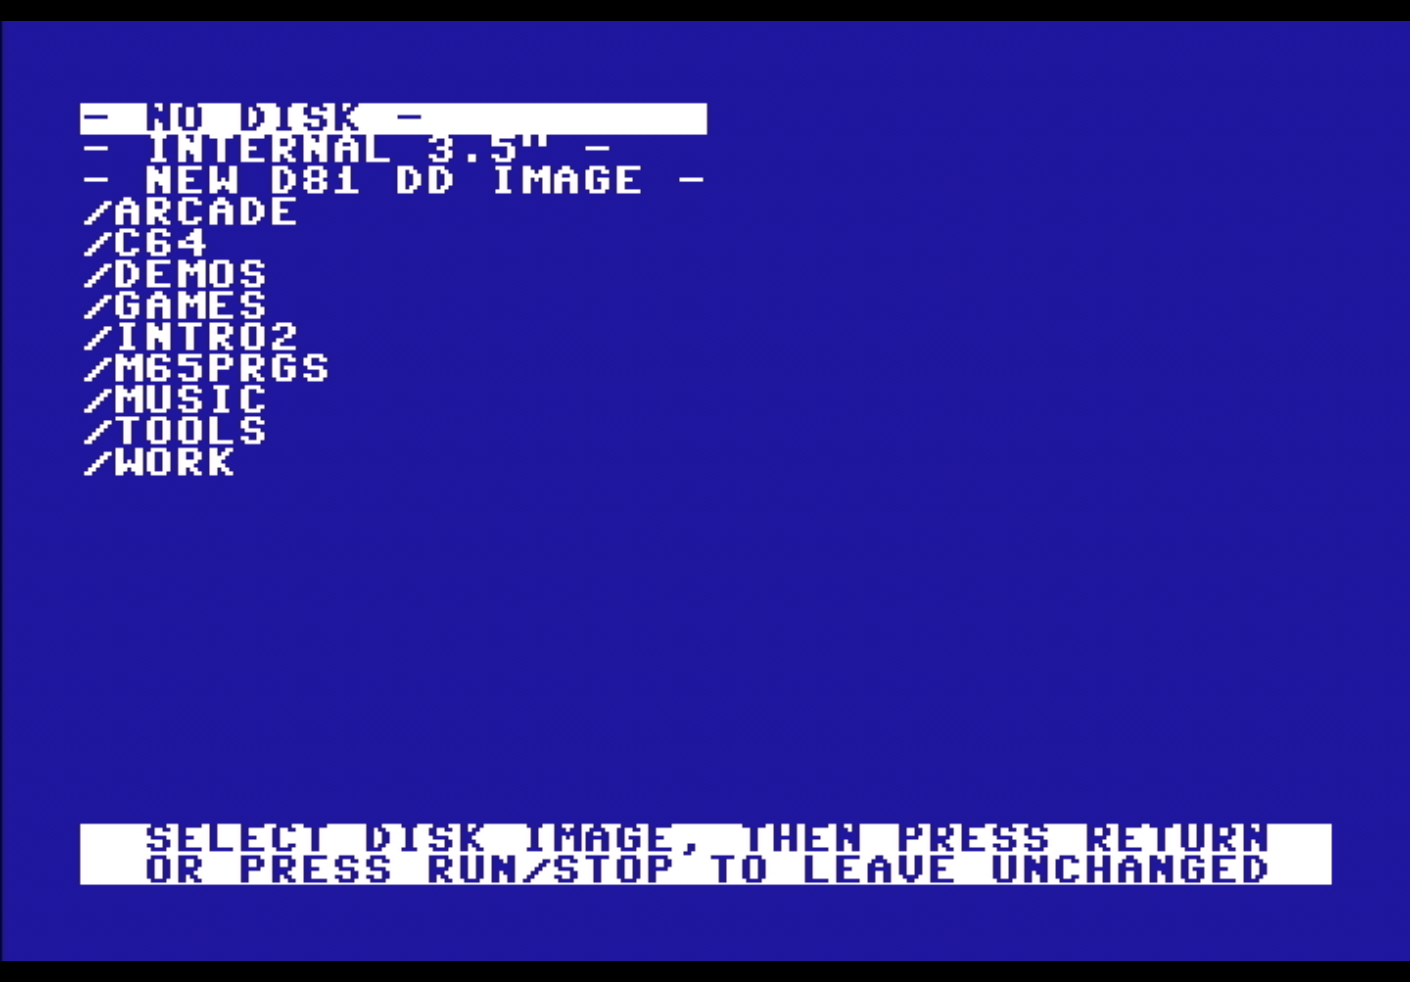
\includegraphics[width=0.7\linewidth]{images/d81-subfolders.png}
\end{center}

You can also create new disk images in sub-directories by navigating to the sub-directory before selecting \screentext{- NEW D81 DD IMAGE -}.

The MEGA65 maintains a ``current working directory'' that is used as the base directory for BASIC commands like {\bf MOUNT}. To change the current working directory from BASIC, using the {\bf CHDIR} command with the {\bf U12} argument:

\begin{screenoutput}
CHDIR "DEMOS",U12

MOUNT "XANADU.D81"
\end{screenoutput}


\section{Using the Internal 3.5" Floppy Disk Drive}

The MEGA65 has a built-in 3.5" floppy disk drive, similar to what was intended for the Commodore 65. You can use physical floppy disks to store your programs and data. Some MEGA65 software can be purchased on floppy disk.

The internal 3.5" drive must be mounted before it can be used. It can be mounted to unit 8 or unit 10.

\subsection{Mounting the 3.5" Drive with the Freezer}

Open the Freezer menu: hold \widekey{RESTORE} for one second, then release it. Notice the current drive mounting settings in the lower-right of the screen.

Press \megakey{0}, then use the cursor down key to: \screentext{- INTERNAL 3.5" -} Press \widekey{RETURN} to select it. The Freezer menu screen shows that the internal drive is mounted to the first managed disk device.

The \screentext{UNIT \#} for the first device can be either 8 or 10. Press \megakey{8} to toggle between these options. BASIC disk commands default to unit 8, so it is typical to use unit 8 unless you are working with multiple disks at the same time.

The internal 3.5" drive cannot be mounted to the second managed drive with unit numbers 9 or 11.

\subsection{Mounting the 3.5" Drive from BASIC}

You can mount the internal 3.5" disk drive to unit 8 using the BASIC {\bf MOUNT} command. This command works from either the \screentext{READY} prompt or from a program. To mount the internal drive to unit 8, enter the command without arguments:

\begin{screenoutput}
MOUNT
\end{screenoutput}

The {\bf MOUNT} command can only mount the internal drive to unit 8. You can only mount it to unit 10 from the Freezer menu.

\subsection{DD vs. HD disks}

The MEGA65 disk controller expects a Double Density (DD) floppy disk in the internal 3.5" floppy disk drive.\footnote{It may be possible to support full-capacity HD disks in a future firmware update. This is not a limitation of the drive hardware.} Floppy disks are no longer manufactured, and the DD variety can be difficult to find.

You can use a High Density (HD) floppy disk with the drive, with one important modification: you must cover the hole in the upper-left corner of the disk with a small piece of opaque tape, such as masking tape. This convinces the drive that the disk is DD, and switches it to a mode compatible with the MEGA65 disk controller.

\begin{center}
  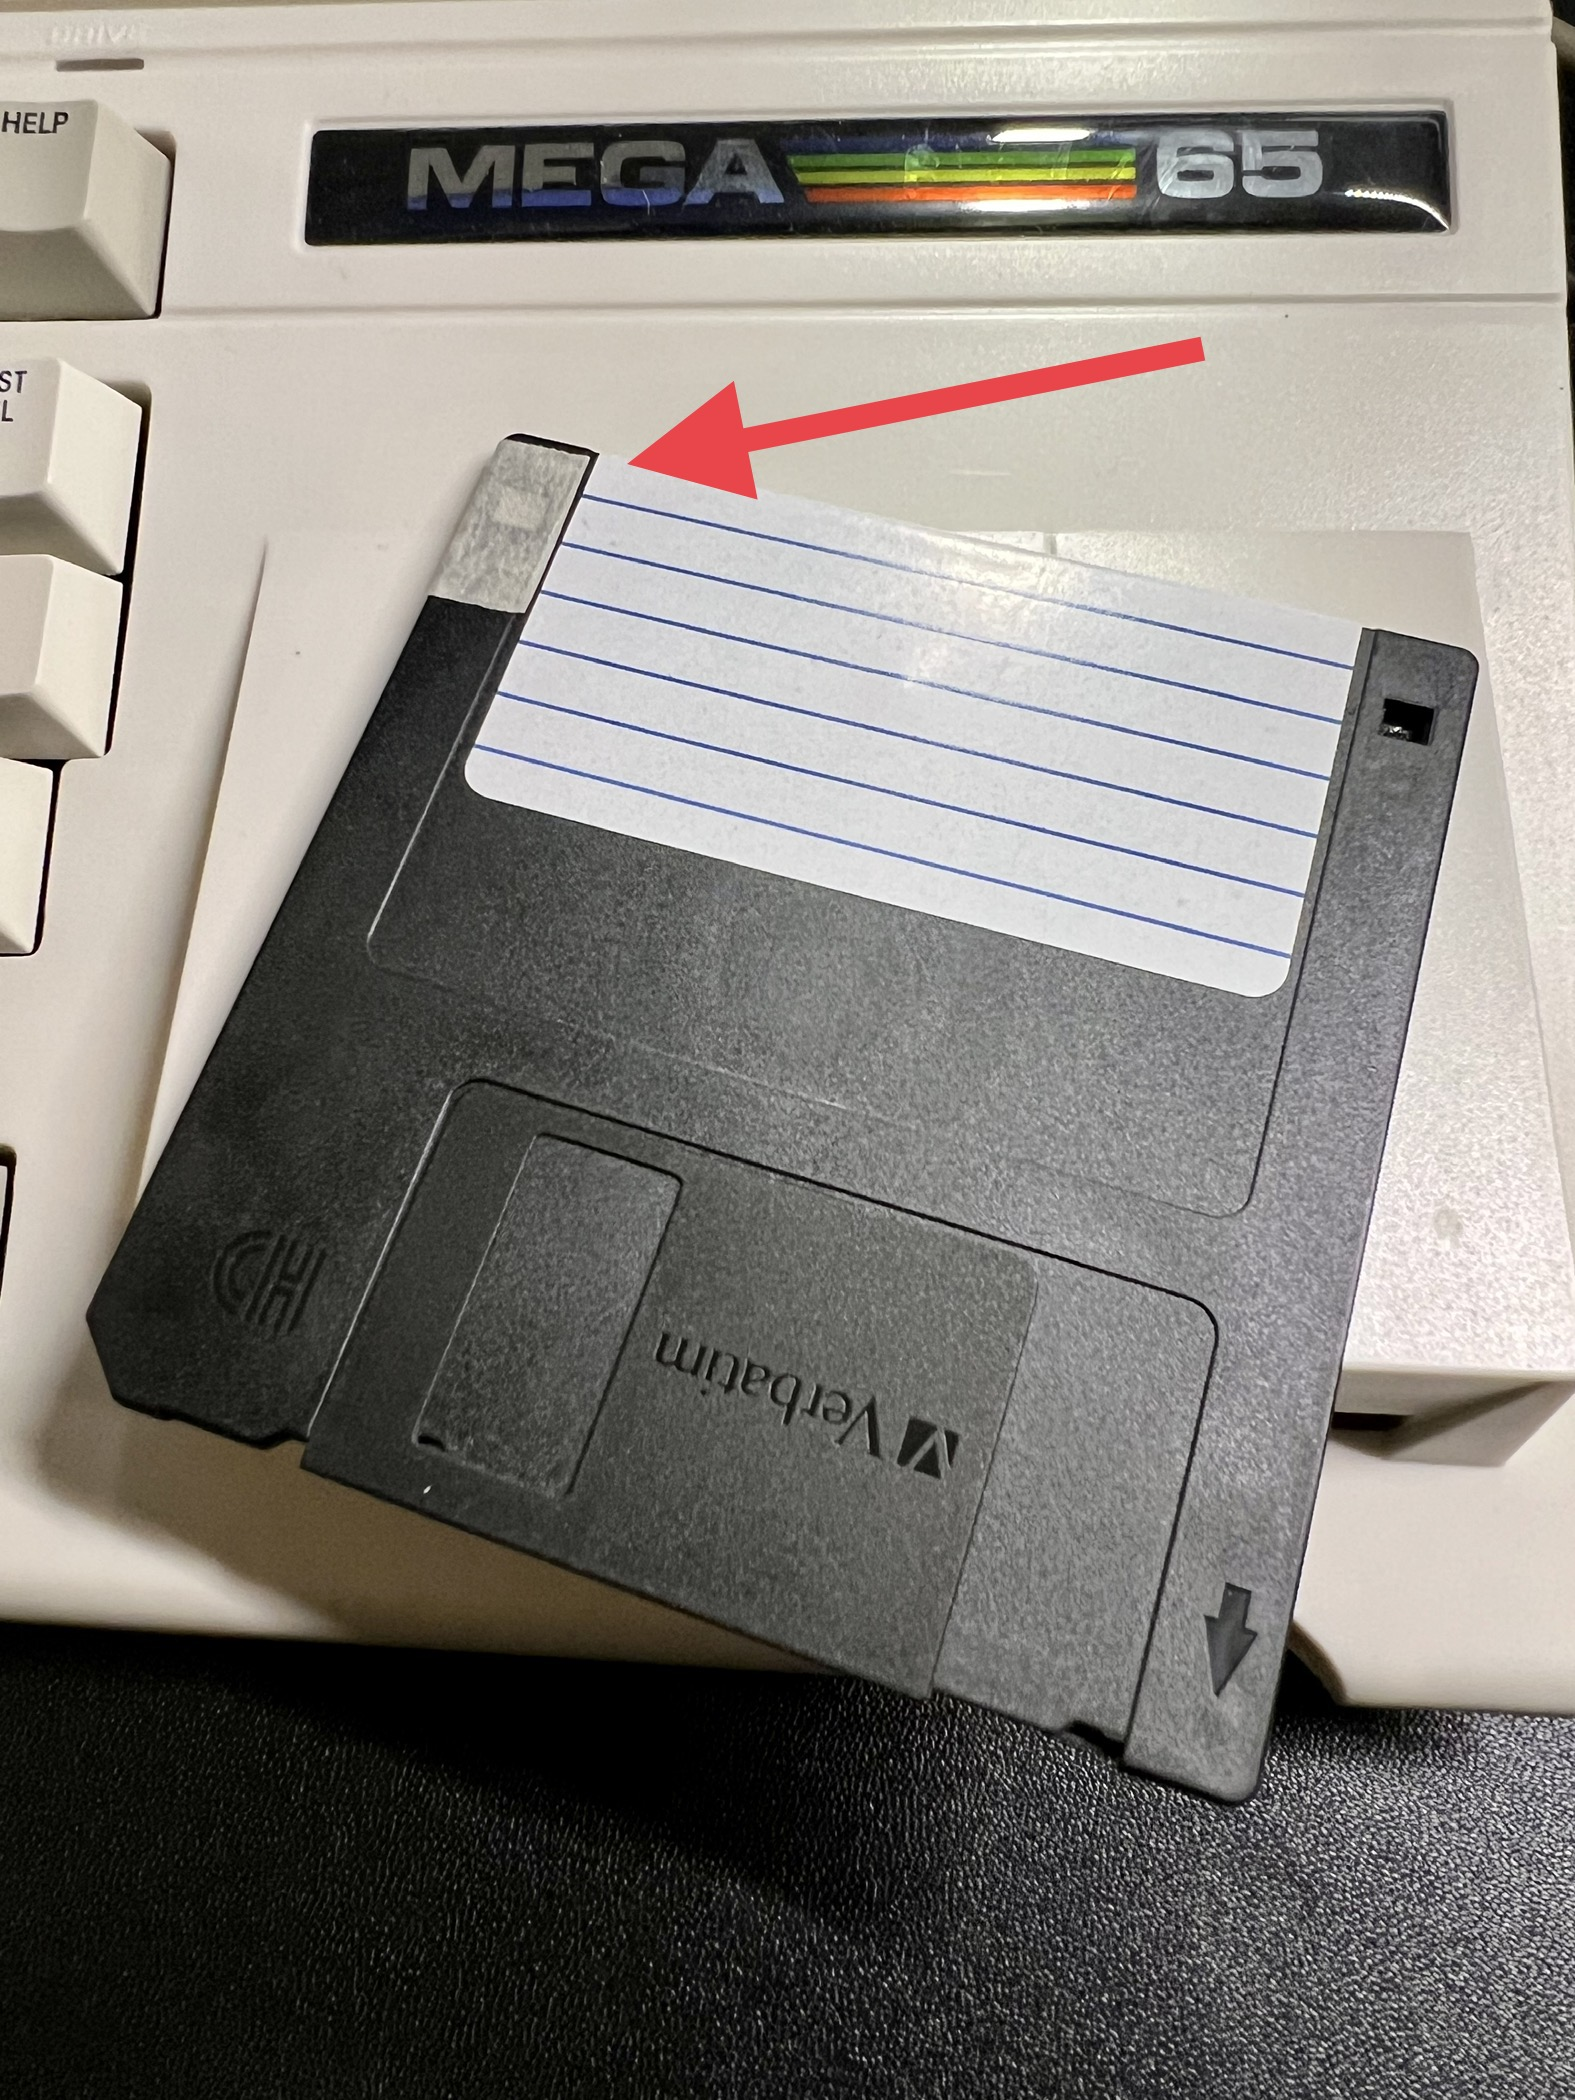
\includegraphics[width=0.7\linewidth]{images/floppy_hd.jpg}
\end{center}

\underline{Note}: Make sure that the tape is opaque, such as masking tape (not Scotch tape), and that it covers both sides of the hole.

\subsection{Formatting a Disk}

A floppy disk must be formatted before it can be used. The MEGA65's internal 3.5" floppy drive emulates a Commodore 1581 drive, and can use disks formatted in such a drive. You can also format a disk with the MEGA65.

\underline{Note}: Formatting a disk erases its contents. Be careful to only do this when you do not need the data on the disk!

To format a physical 3.5" floppy disk using the internal drive:

\begin{enumerate}
\item Open the Freezer.
\item Mount the internal 3.5" floppy drive to the first managed drive slot, unit 8.
\item {\it Double-check that unit 8 says:} \screentext{- INTERNAL 3.5" -}
\item Resume the computer: press \megakey{F3}.
\item Insert the floppy disk you wish to format into the internal floppy drive.
\item Enter the BASIC {\bf FORMAT} command, giving it a name ({\tt "MYDISK"}) and a two-character ID ({\tt XX}).
\begin{screenoutput}
FORMAT "MYDISK",IXX
\end{screenoutput}
\item When prompted, enter {\tt YES} and press \widekey{RETURN}.
\end{enumerate}

Formatting the disk takes a minute or so. The drive will make buzzing and clicking noises during the process. Do not switch off the computer or eject the disk until formatting is complete.

You can confirm that the formatting was successful by issuing the {\bf DIR} command. You should see an empty directory listing with the name and ID you specified. Your disk is now ready to use.


\section{Using External IEC Disk Drives}

The MEGA65 works with external disk drives connected to the IEC serial port.

External drives do not need to be mounted. If a unit number is not assigned to the internal 3.5" disk drive or to a disk image, disk operations intended for that unit number will be transmitted to the IEC serial port. It is up to the device connected to the port to recognize its unit number. Some IEC devices have switches that let you set the unit number. Others will only work with a specific number.

If you have an external drive that expects a specific unit number, you will need to make sure the MEGA65 isn't assigning that number to a disk image or the internal drive. Open the Freezer, then press \megakey{8} or \megakey{9} to toggle the unit number assignments so that they no longer use the needed unit number.

The drive and unit assignments are temporary, and will be reset to their defaults when the MEGA65 is switched off. You will need to re-configure the drive assignments the next time you switch on the computer.


\section{Bootable Disks}

With older Commodore computers, it was common for software makers to organize the file directory on a floppy disk such that the first file in the list is the main program. The user could then enter the command \screentext{LOAD "*",8,1} to load the main program, and \screentext{RUN} to run it. The asterisk is a wildcard that matches any file, so it matches the first file on the disk, without the user having to type the name of the program.

This method is still common, and the MEGA65 has a quick way to boot such disks: hold \specialkey{SHIFT} and press \specialkey{RUN STOP}. This executes the \screentext{RUN "*"} command, which is similar to the familiar command sequence that loads and runs the first program on the disk.

With the C65, Commodore introduced a new way to boot disks. Instead of relying on file order, a disk can have a file named {\tt AUTOBOOT.C65}. If this file exists and is a program, the BASIC {\bf BOOT} command will load and run this file.

\begin{screenoutput}
BOOT
\end{screenoutput}

\subsection{Auto-Booting Disks}

As discussed in chapter \vref{cha:configuringyourmega}, you can use the Configuration Utility to set the MEGA65 to mount either a virtual disk image or the internal 3.5" disk drive automatically during boot. (You can also disable this feature by selecting the virtual disk, then leaving the field that asks for the disk image name empty.)

If the mounted disk is bootable---that is, it contains a program file named {\tt AUTOBOOT.C65}---the MEGA65 will load and run the boot program automatically.

This is how the Intro Disk works. The Intro Disk menu is a program named {\tt AUTOBOOT.C65} on the virtual disk image {\tt MEGA65.D81}, which is pre-configured to be the mounted disk on system start-up. When you disable the Intro Disk from its menu, it renames {\tt AUTOBOOT.C65} to {\tt MENU}, such that the disk is no longer considered bootable.

Setting up a boot disk for yourself can be a handy way to configure your computer. You can write a short BASIC program that changes the system font, adjusts the background color, and sets {\bf KEY} macros to your taste, then save the program as {\tt AUTOBOOT.C65} on a disk that you have configured to mount on system start-up. This program will run every time you switch on your MEGA65.


\section{Accessing the SD Card from BASIC}

Several BASIC 65 commands can operate directly on the MEGA65 SD card as if it were a disk drive. In these cases, the SD card is known as unit 12.

\underline{Note}: Unit 12 can only be accessed directly for a few specific operations. It cannot treat the entire SD card as if it were a CBDOS disk.

To list all of the files on the SD card, use the {\bf DIR} command with the \screentext{U12} argument:

\begin{screenoutput}
DIR U12
\end{screenoutput}

To load or save a PRG file directly from the SD card (that isn't in a D81 disk image), use the \screentext{U12} argument with the {\bf DLOAD} and {\bf DSAVE} commands. You {\em must} include the {\tt .PRG} filename suffix in this case, which is different from using PRG files on disks or disk images.

\begin{screenoutput}
DLOAD "MYPROGRAM.PRG",U12
\end{screenoutput}

As shown earlier, the MEGA65 supports sub-directories (sub-folders) on the SD card, and maintains a current working directory for disk operations. To change the current working directory to a subdirectory:

\begin{screenoutput}
CHDIR "SUBDIR",U12
\end{screenoutput}

To change the current working directory to the parent of the current directory:

\begin{screenoutput}
CHDIR "..",U12
\end{screenoutput}

The {\bf MOUNT} command can mount a D81 disk image to a unit number. Even though this command refers to a file on the SD card, it does not use the \screentext{U12} argument. Instead, it uses the {\bf U} argument to select the unit number for the disk being mounted. The {\bf MOUNT} command does use the current working directory set by {\bf CHDIR} to locate the file.


\section{Common Disk Operations}

The following are some examples of common disk operations you can perform at the \screentext{READY} prompt. See the BASIC command reference in appendix \vref{cha:basic-reference} for more information.

Most commands that accept filenames also accept a {\bf U} argument that says which unit has the file. The default unit is 8.\footnote{The default disk unit for BASIC commands starts out as 8. You can change it with the {\bf SET DEF} command.}

\subsection{DIR}

To display the directory (list of files) for a disk, use the {\bf DIR} command.

\begin{screenoutput}
DIR

DIR U9
\end{screenoutput}

Unlike the Commodore 64 method of loading the disk directory into BASIC memory, the {\bf DIR} command does not modify BASIC memory. It is safe to use {\bf DIR} with a program in memory.

To make larger directories easier to view, {\bf DIR W} (for ``wide'') displays the directory in columns, pausing for each page.

\subsection{DLOAD and RUN}

The {\bf DLOAD} command loads a program from disk into memory. The {\bf RUN} command runs the program currently in memory.

\begin{screenoutput}
DLOAD "COOLGAME"
RUN
\end{screenoutput}

You can combine these into one command by providing the filename directly to the {\bf RUN} command.

\begin{screenoutput}
RUN "COOLGAME"
\end{screenoutput}

\subsection{DSAVE}

The {\bf DSAVE} command saves the BASIC program currently in memory to disk.

\begin{screenoutput}
DSAVE "MYGAME"
\end{screenoutput}

By default, this will refuse to overwrite an existing file with the same name. To request that the existing file be overwritten, put an {\tt @} (at) symbol before the filename, inside the double-quotes.

\begin{screenoutput}
DSAVE "@MYGAME"
\end{screenoutput}

Note that save-with-replace is only recommended when using disk images and the 3.5" floppy drive. Older Commodore drives had bugs in this feature that could result in data loss.

\subsection{BACKUP}

The {\bf BACKUP} command copies an entire disk from one unit to another. All existing data on the destination disk is erased as part of this process.

\begin{screenoutput}
BACKUP U8 TO U9
\end{screenoutput}

You can use {\bf BACKUP} to make disk images from floppy disks, or write disk images to floppy disks, or copy everything from one disk drive to another.

\subsection{COPY}

The {\bf COPY} command makes a copy of a file. If the source and the destination are different filenames on the same unit, this duplicates the file on the disk.

\begin{screenoutput}
COPY "MYGAME",U8 TO "MYGAME",U9

COPY "MYGAME" TO "MYGAME-V1"
\end{screenoutput}

\subsection{RENAME}

The {\bf RENAME} command changes the name of an existing file.

\begin{screenoutput}
RENAME "MYGAME-V29" TO "MYGAME-FINAL"
\end{screenoutput}

\subsection{DELETE}

The {\bf DELETE} command deletes a file.

\begin{screenoutput}
DELETE "JUNKFILE"
\end{screenoutput}


\subsection{Shortcut Disk Commands}

BASIC 65 provides several shortcuts for common disk commands for use from the \screentext{READY} prompt.

\begin{center}
\begin{tabular}{|l|l|}
\hline
{\bf Shortcut} & {\bf Equivalent Command} \\
\hline
\screentextwide{/} & {\bf LOAD} \\
\hline
$\uparrow$ & {\bf RUN} \\
\hline
$\leftarrow$ & {\bf SAVE} \\
\hline
\screentextwide{@} & {\bf DISK} \\
\hline
\screentextwide{\$} & {\bf DIR} \\
\hline
\end{tabular}
\end{center}

These are intended to be used with a directory listing to launch programs without having to type filenames. For example:

\begin{enumerate}
\item Display the disk's directory listing: type {\bf \$}, press \widekey{RETURN}.
\item Use the cursor keys to move the cursor to the line with the program you want to run.
\item Type {\bf \screentext{$\uparrow$}}, press \widekey{RETURN}.
\end{enumerate}

The selected program loads and runs. Notice that you do not have to clear extra characters from the line. The shortcut knows to ignore everything but the filename in double-quotes, as printed by the directory listing.
